\chapter{Strumenti numerici indicatori - parte I}

\begin{figure}[h]
    \centering
    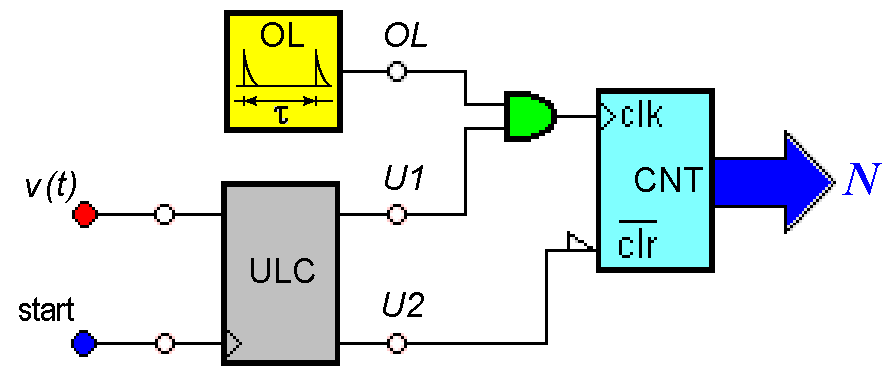
\includegraphics[scale = 0.5]{OL GATE CNT.png}
\end{figure}

\newpage 

\section{Pregi della misura numerica}
\footnote{Slide della prof | SDME 4 Strumenti numerici indicatori - parte I | pag 2 \\  
Appunti | 2025-04-11 | pag 2}

Per misurazione numerica si intende quel processo di misura in cui alla fine si ha un numero. \newline 

Prima dell'avvento del digitale, nel nostro ambito degli strumenti digitali, quindi delle misurazioni numeriche, 
si utilizzavano gli strumenti analogici come il seguente: 

\begin{figure}[h]
    \centering
    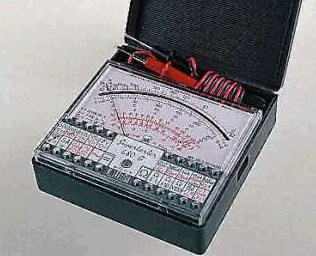
\includegraphics[scale = 0.5]{Strumento analogico di esempio.png}
\end{figure}

che, in base alla bravura dell'operatore, erano possibili definire delle misure attendibili. \newline 

Sono due i principali pregi della misurazione numerica: 

\begin{itemize}
    \item facilità di lettura 
    \item possibilità di elaborazione
\end{itemize}

Per facilità di lettura si intende che uno strumento fornisce il valore della misurazione in forma
numerica , così da essere più agevole e leggibile rispetto ad uno strumento analogico. \newline 

Basta notare la misurazione di tensione da un voltmetro digitale: 

\begin{figure}[h]
    \centering
    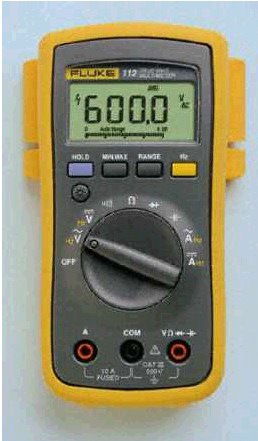
\includegraphics[scale = 0.4]{Fluke 112.png}
\end{figure}

Per possibilità di elaborazione si intende che gli strumenti numerici possono utilizzare il microprocessore per eseguire elaborazioni anche complesse 
sul segnale misurato, e possono registrare le informazioni su supporti digitali, come il caso 
dei moderni oscilloscopi digitali: 

\begin{figure}[h]
    \centering
    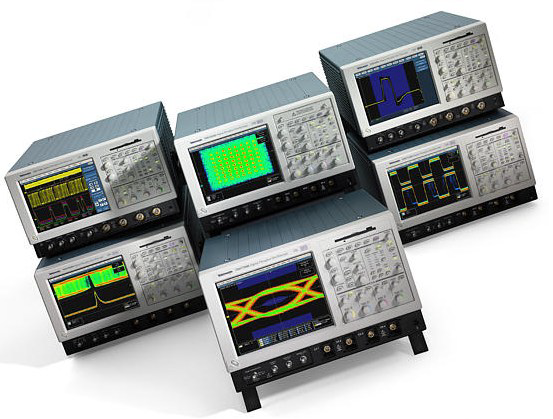
\includegraphics[scale = 0.4]{oscilloscopi digitali.png}
\end{figure}

\newpage

\section{Limiti della misura numerica}
\footnote{Slide della prof | SDME 4 Strumenti numerici indicatori - parte I | pag 3 \\  
Appunti | 2025-04-11 | pag 2 - 3}

Il misurando è solitamente una grandezza che varia in modo continuo, mentre il processo di misurazione numerica 
fornisce un valore che è costituito da un numero "intero": questo processo prende il nome di quantizzazione, che è dovuto dalla natura dello strumento 
di misura digitale, quindi discretizzato. \newline 


Il parametro misurato dallo strumento di misura digitale è espresso come somma di elementi indivisibili, cioè i quanti, e ciò determina una inevitabile perdita di informazione. \newline 

Facendo la quantizzazione, quindi la discretizzazione, del segnale non si potrà ritornare indietro al segnale analogico originale che contiene infiniti valori. \newline 

Il massimo che si può fare è aumentare i quanti, cioè aumentare il contatore, quindi la dimensione del registro dello strumento di misura. \newline 

\newpage 

\subsection{Incertezza di quantizzazione}
\footnote{Slide della prof | SDME 4 Strumenti numerici indicatori - parte I | pag 4 \\  
Appunti | 2025-04-11 | pag 3}

Per ridurre la perdita di informazione dovuta alla quantizzazione, si devono usare quanti più piccoli. \newline 

Facendo un confronto tra segnale analogico e digitale: 

\begin{figure}[h]
    \centering
    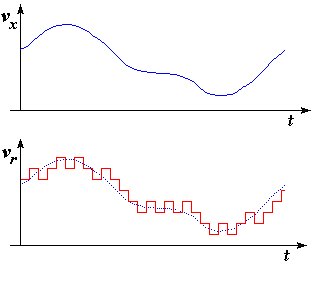
\includegraphics[scale = 1]{Segnale analogico e segnale quantizzato.png}
\end{figure}

Il segnale in rosso è quello quantizzato: se i quanti diventassero infiniti, il segnale rosso e quello analogico si sovrapporrebbero. \newline 

\newpage 

\section{Dimensione dei quanti e capacità del contatore}
\footnote{Slide della prof | SDME 4 Strumenti numerici indicatori - parte I | pag 5 \\  
Appunti | 2025-04-11 | pag 3 - 4}

Consideriamo un esempio di due tester che hanno la stessa portata, ma quanti di dimensione differente: 

\begin{figure}[h]
    \centering
    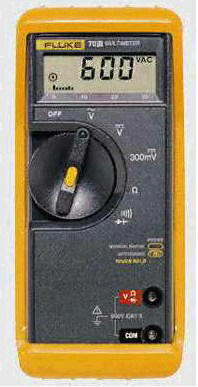
\includegraphics[scale = 1]{Voltmetro con quanto da 1 volt.png}
    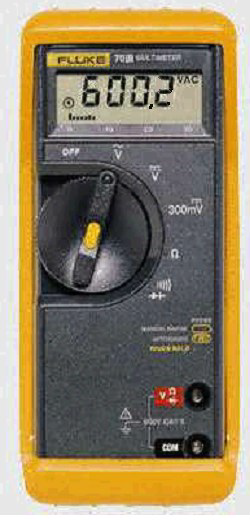
\includegraphics[scale = 0.75]{Voltmetro con quanto da 0,1 volt.png}
\end{figure}

In questo esempio, i due voltmetri misurano lo stesso misurando, ma quello a sinistra presenta 600 quanti, 
ogni quanto misura 1 volt, 
nel contatore è presente il numero 600, quindi sarà necessario almeno un registro a 10 bit. \newline 

Invece il voltmetro a destra ha 6002 quanti, in cui ogni quanto misura 0.1 volt, nel registro è presente il numero 6002, 
quindi un registro grande almeno 13. \newline 

Di seguito una tabella che indica la grandezza del registro in bit e il numero di quanti che può contenere: 

\begin{figure}[h]
    \centering
    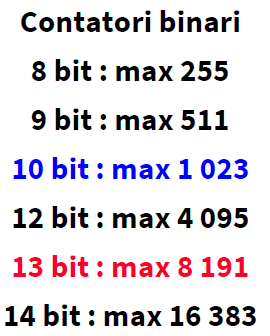
\includegraphics[scale = 0.6]{Da bit a numeri.PNG}
\end{figure}

Essendo degli strumenti di misura, gli ADC sono presenti negli strumenti digitali. \newline

Nelle architetture degli strumenti, ADC e contatore devono lavorare insieme, a "braccetto", allo stesso tempo e in sincronia. \newline 

\newpage 

\section{Parte I: Intervallometro e periodometro}
\footnote{Slide della prof | SDME 4 Strumenti numerici indicatori - parte I | pag 6 - 7 \\  
Appunti | 2025-04-11 | pag 4 - 5}

Parlando di contatori e ADC, per lavorare insieme allo stesso tempo è necessario intervallare il tempo in modo costante. \newline

Per questo sono utili, in uno strumento di misura, l'intervallometro e periodometro. \newline 

Essendo presenti in uno strumento numerico, si considerano intervallometro e periodometro numerici. \newline 

L'intervallometro numerico è quello strumento per la misura di arbitrari intervalli di tempo. \newline 

Il periodometro numerico è quello strumento che misura anch'esso la durata di un intervallo di tempo, 
ma, in particolare, la durata del periodo di un segnale ripetitivo, cioè periodico. \newline 

Con l'aggiunta di un trigger in ingresso, si può ottenere un periodometro da un intervallometro. \newline 

Andando nello specifico, con l'intervallometro si misura la durata del $T_{on}$ di un segnale elettrico "binario", cioè per quanto tempo il segnale resta a livello alto. \newline 

Considerando un segnale qualsiasi, anche analogico, con un intervallometro si misura la durata tra $t_2 - t_1$ di un intervallo che separa due eventi riconosciuti da un circuito di trigger. \newline 

\begin{tcolorbox}
    Generalmente, la durata $t_2 - t_1$ viene scelta da noi    
\end{tcolorbox}

Con il circuito di trigger si potrà costruire un segnale di servizio che abbia un $T_{on}$ pari alla durata dell'intervallo che va da $t_1$ a $t_2$ che vogliamo misura. \newline 

Il segnale di trigger non sarà soggetto di misura, è solo di servizio. \newline 

Invece con il periodometro si può misurare il periodo T di un segnale elettrico analogico e periodico. \newline 

Un segnale si definisce periodico se: 

{
    \Large 
    \begin{equation}
        g(t) = g(t- n T) \forall t \in \real, \forall n \in \mathbb{Z} 
    \end{equation}
}

\newpage 


\begin{tcolorbox}
    Ora è il momento delle famose slide in cui non c'è scritto nulla e bisogna spiegare tutto quello che si è preso come appunti a lezione. \newline 
    
    Queste architetture, come altre, verranno richieste in dettaglio all'esame. 
\end{tcolorbox}

\section{Intervallometro: principio di misurazione}
\footnote{Slide della prof | SDME 4 Strumenti numerici indicatori - parte I | pag 8 \\  
Appunti | 2025-04-11 | pag 5 - 7}

Come si fa a misurare la durata di un intervallo di tempo? \newline 

L'intervallo di tempo deve essere costante. \newline 

Considerando i grafici di start della misura, oscillatore locale OL, e quello del clock clk: 

\begin{figure}[h]
    \centering
    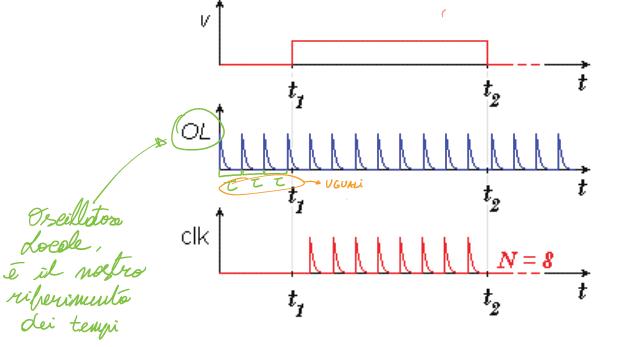
\includegraphics[scale = 0.8]{servizio OL e clk con appunti.PNG}
\end{figure}

si può notare che nell'intervallo $[t_1, t_2]$ si rivelano N impulsi, generati da un campione di tempo, 
distanziati di un periodo $\tau$. \newline 

Allora, la durata dell'intervallo è data da: 

{
    \Large 
    \begin{equation}
        t_2 - t_1 = N \tau
    \end{equation}
}

Da questa formula, si deduce che il tempo misurato è razionale. \newline 

Per contare quanti N impulsi sono stati emessi dall'OL è necessario un contatore, quindi un registro. \newline

Inoltre, come si può notare dalle figure, non si può misurare sotto al tempo di $\tau$. \newline 

L'OL riesce a generare impulsi costanti nel tempo grazie alle proprietà di alcuni circuiti e materiali (che non andremo ad analizzare in questo corso), 
in particolare alla proprietà piezoelettrica del quarzo. \newline 

\begin{tcolorbox}
    Fun fact successo a lezione. \newline 
    
    La prof dice: "Se tu dai un cazzotto forte al quarzo, lui genera un segnale costante nel tempo". \newline 

    Se vuoi approfondire meglio e non vuoi dare cazzotti alle pietre perchè, come dice Squartini, "noi facciamo parte del partito della non violenza", ti lascio il link \newline 

    \url{https://www.chimica-online.it/download/piezoelettricita.htm}
\end{tcolorbox}


\newpage 

\section{Intervallometro numerico: schema di principio}
\footnote{Slide della prof | SDME 4 Strumenti numerici indicatori - parte I | pag 9 \\  
Appunti | 2025-04-11 | pag 7}

Ecco a voi lo schema di principio di un intervallometro numerico: 

\begin{figure}[h]
    \centering
    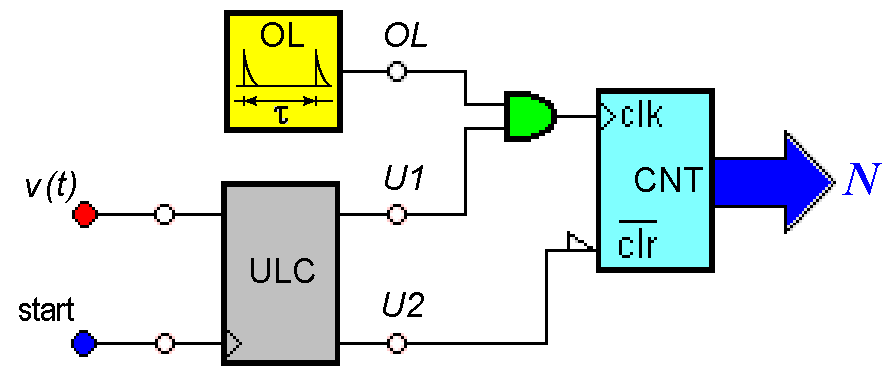
\includegraphics[scale = 0.6]{OL GATE CNT.png}
\end{figure}

\begin{tcolorbox}
    Come detto a lezione, se si vuole intervallare il tempo avremo bisogno sempre almeno di: 
    \begin{itemize}
        \item Oscillatore 
        \item Gate 
        \item Contatore
    \end{itemize}

    Queste tre parole ci devono entrare dentro il cervello meglio dell'Ave Maria: ve lo ripeterete la notte
\end{tcolorbox}

Lo schema di principio di un intervallometro numerico è composto da: 

\begin{itemize}
    \item Oscillatore Locale OL (in figura il blocco giallo) 
    \item Gate, cioè una porta logica AND dove il segnale di usita è alto se tutti e due gli ingressi sono a livello alto (indicato nella figura di verde) 
    \item Unità logica di controllo ULC, cioè il "cervello" dell'intervallometro (in figura il blocco grigio) 
    \item Contatore CNT, che nella realtà sarà un registro (in figura il blocco celestino) 
\end{itemize}

Alcune osservazioni riguardo il contatore. \newline 

Il contatore CNT ha due pin: 

\begin{itemize}
    \item clock (clk), che è sensibile ai fronti di salita 
    \item pin clear negato ($\overline{clr}$), che è sensibile ai fronti di discesa  
\end{itemize}

Per evitare il cross-talk tra la linea di $\overline{clr}$ e clk, la sensibilità dei fronti è opposta. \newline 

Il contatore CNT è proprio quel registro che conta gli impulsi $\tau$ dall'oscillatore locale OL della formula: 

{
    \Large 
    \begin{equation}
        t_2 - t_1 = N \tau
    \end{equation}
}

\newpage 

\subsection{Principio di funzionamento}
\footnote{Slide della prof | SDME 4 Strumenti numerici indicatori - parte I | pag 10 \\  
Appunti | 2025-04-11 | pag 7 - 10 | 2025-04-15 | pag 2}

Di seguito lo schema a blocchi e le funzioni nel tempo dell'intervallometro numerico: 

\begin{figure}[h]
    \centering
    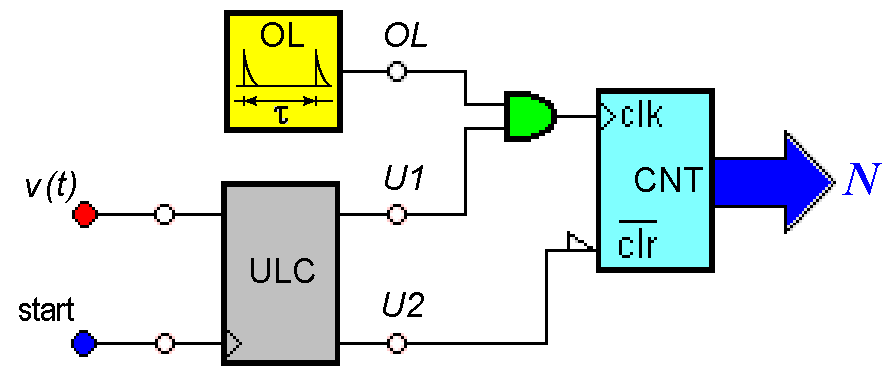
\includegraphics[scale = 0.6]{OL GATE CNT.png}
    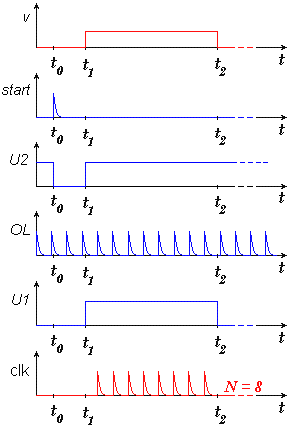
\includegraphics[scale = 1]{tensioni dei segnali in un intervallometro numerico.png}
\end{figure}

\begin{tcolorbox}
    Possono far impressione per la prima volta i grafici, ma alla fine il funzionamento è molto semplice
\end{tcolorbox}

Il procedimento dell'intervallometro inizia al tempo $t_0$ in cui, come si vede dal grafico del pin start, 
c'è un fronte di salita dello start. \newline 

Il segnale di start viene mandato all'ULC, che a sua volta, manda il segnale di clear al CNT. \newline 

Il grafico che visualizziamo del pin U2 dobbiamo considerarlo al contrario perchè al CNT si considera il negato del clr, 
quindi se noi visualizziamo tra $t_1$ e $t_2$ nel pin U2 il livello basso, il CNT lo interpreta come livello alto. \newline 

Quando il CNT ha pulito il registro, si può iniziare il processo di misura, cioè dall'istante $t_1$. \newline 

L'ULC imposta ad alto il pin U1 per un periodo che va da $t_1$ a $t_2$ e che viene scelto dall'ULC. \newline 

Il tempo $t_2 - t_1$ è lo stesso indicato nella formula precedente con $N\tau$: 

{
    \Large 
    \begin{equation}
        t_2 - t_1 = N \tau
    \end{equation}
}

L'OL non dipende da altri pin del circuito: lui continua ad inviare impulsi in modo indefinito. \newline 

I pin U1 e OL sono di ingresso al gate AND, che, come sappiamo dalla tabella di verità dell'AND, 
diventa alto quando tutti e due gli ingressi sono alti. \newline 

L'uscita del gate è collegato al pin clk del CNT. \newline 

Quindi, quando c'è un fronte di salita del clock, il CNT aggiorna il suo registro e lo incrementa ogni colpo di clk dell'OL, se il pin U1 è a livello alto. \newline 

Quando l'ULC manda al pin U1 un livello basso, nella figura dal tempo $t_2$ in poi, 
il CNT si ferma ai valori di clock precedentemente contati. \newline 

Il processo di funzionamento dell'intervallometro rinizia da capo quando si rimanda un segnale di start e si pulisce il CNT. \newline 

\newpage 

\subsection{Incertezza}
\footnote{Slide della prof | SDME 4 Strumenti numerici indicatori - parte I | pag 10 \\  
Appunti | 2025-04-11 | pag 7 - 10}

Siccome siamo in ambito misuristico, bisogna studiare l'architettura sotto l'aspetto dell'incertezza. \newline 

Sappiamo che: 

{
    \Large 
    \begin{equation}
        t_2 - t_1 = N \tau
    \end{equation}
} 

dove N è un numero intero. \newline 

Come ci dice la GUM, svolgendo le derivate parziali della formula per le due grandezze che consideriamo statisticamente indipendenti, 
si può calcolare l'incertezza di $t_2 - t_1$ come: 

{
    \Large 
    \begin{equation}
        \frac{\Delta (t_2 - t_1)}{t_2 - t_1}
        = 
        \frac{\Delta \tau}{\tau} 
        + 
        \frac{\Delta N}{N}
    \end{equation}
}

L'obbiettivo, come ogni ambito nelle misure, è rendere l'incertezza, cioè $\frac{\Delta (t_2 - t_1)}{t_2 - t_1}$ la più bassa possibile. \newline 

Dal punto di vista ingegneristico, e quindi non matematico, il contributo di incertezza legato a $\tau$, 
cioè $\frac{\Delta \tau}{\tau}$, non si può migliorare perchè è legato all'oscillatore locale. \newline 

\begin{tcolorbox}
    Tecnicamente lo possiamo migliorare, cioè renderlo più basso: sostituendo l'oscillatore locale con un altro, ma molte delle volte questo non è possibile
\end{tcolorbox}

Il contributo $\frac{\Delta N}{N}$ si può migliorare. \newline 

\newpage 


\subsection{La quantizzazione}
\footnote{Slide della prof | SDME 4 Strumenti numerici indicatori - parte I | pag 11 - 13 \\  
Appunti | 2025-04-11 | pag 10 - 11}

Come scritto nella sezione precedente, in questa architettura ci possono essere diversi contributi di incertezza. \newline 

Notando il seguente grafico: 

\begin{figure}[h]
    \centering
    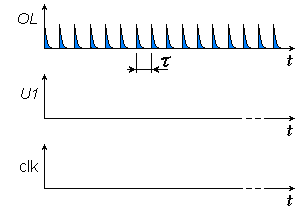
\includegraphics[scale = 1]{1 caso tensioni di esempio nell'intervallometro.png}
\end{figure}

Nell pin di clk del CNT non è presente nulla perchè l'ULC non ha mandato un segnale alto al pin U1, 
quindi il contatore CNT non conta nessun N. \newline 

Invece in questo caso: 

\begin{figure}[h]
    \centering
    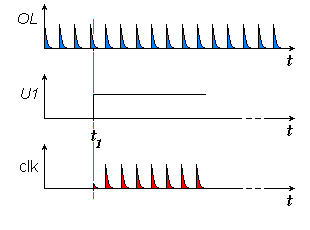
\includegraphics[scale = 1]{2 caso tensioni di esempio nell'intervallometro.png}
\end{figure}

l'ULC, all'istante $t_1$, manda un segnale alto al pin U1, ma, in $t_1$, 
l'OL non ha un fronte di salita, e quindi viene considerato il successivo segnale di clk. \newline 

Per arrivare al pin clk del CNT, l'OL deve trovarsi oltre una certa soglia di tensione prefissata dal pin di clk. \newline 

Oltre a questi due casi, possono accadere anche questi due casi in cui, nonostante il sincronismo, 
vengono comunque contati N = 8 : 

\begin{figure}[h]
    \centering
    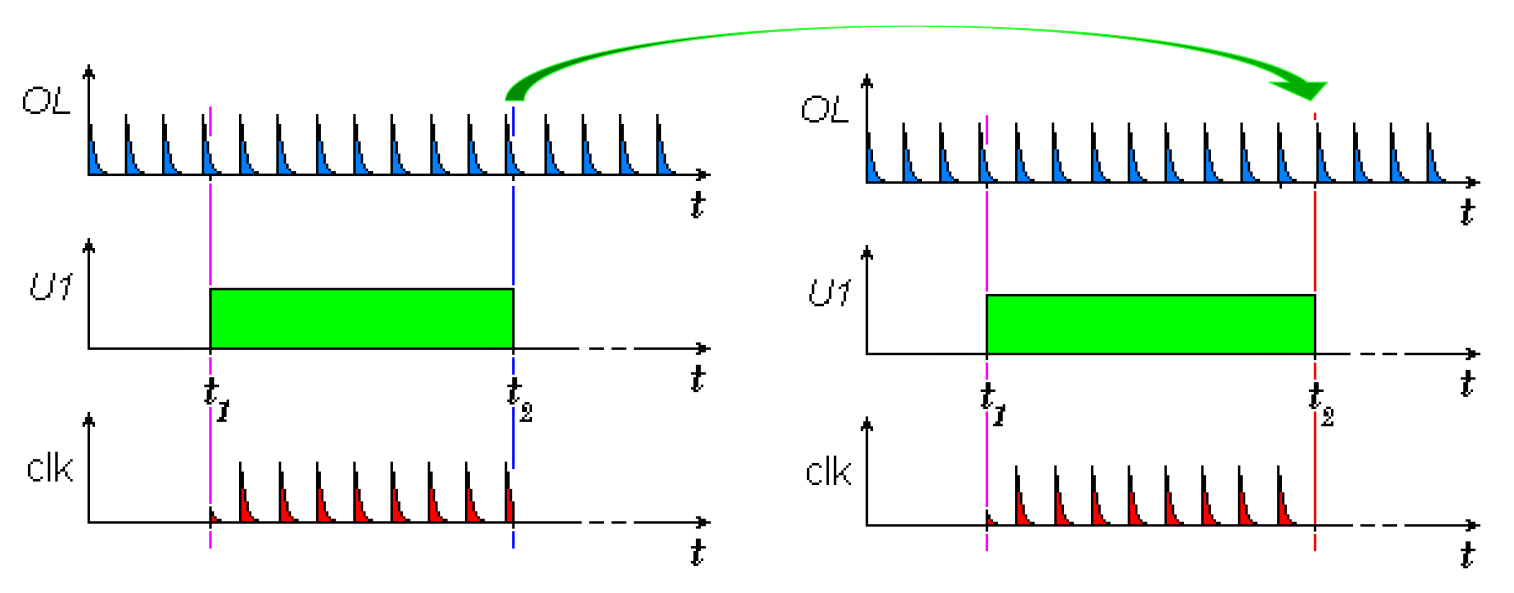
\includegraphics[scale = 0.4]{3 e 4 caso tensioni di esempio nell'intervallometro.png}
\end{figure}

\newpage 

Nella figura a sinistra, al tempo $t_1$, il pin U1 diventa alto, ma l'OL non ha un fronte di salita: 
è troppo basso per il clk per essere contato dal CNT. \newline 

Al tempo $t_2$, il pin U1 diventa basso, ma l'OL ha avuto un fronte di salita un attimo prima che U1 si portasse a zero, 
quindi il segnale di clk è sopra la soglia e viene considerato dal CNT. \newline

Invece, nella figura a destra, al tempo $t_1$ accade la stessa cosa che è accaduto al caso a sinistra. \newline 

All'istante $t_2$, a differenza della figura di sinistra, l'U1 diventa basso prima di un fronte di salita del clk. \newline 

Quindi in tutti e due casi, proprio perchè non si può contare un impulso sotto il tempo di $\tau$, i CNT contano sempre N = 8. \newline 

Questi due fenomeni  si possono giustificare perchè non si può misurare sotto al tempo di $\tau$. \newline 

Un altro caso di N = 8 nonostante la mancanza di sincronismo: 

\begin{figure}[h]
    \centering
    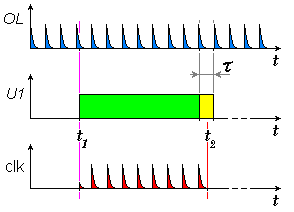
\includegraphics[scale = 1]{5 caso tensioni di esempio nell'intervallometro.png}
\end{figure}

\newpage 

\subsection{Incertezza da mancanza di sincronismo}
\footnote{Slide della prof | SDME 4 Strumenti numerici indicatori - parte I | pag 14 - 15 \\  
Appunti | 2025-04-11 | pag 11 - 12}

Consideriamo questi due casi: 

\begin{figure}[h]
    \centering
    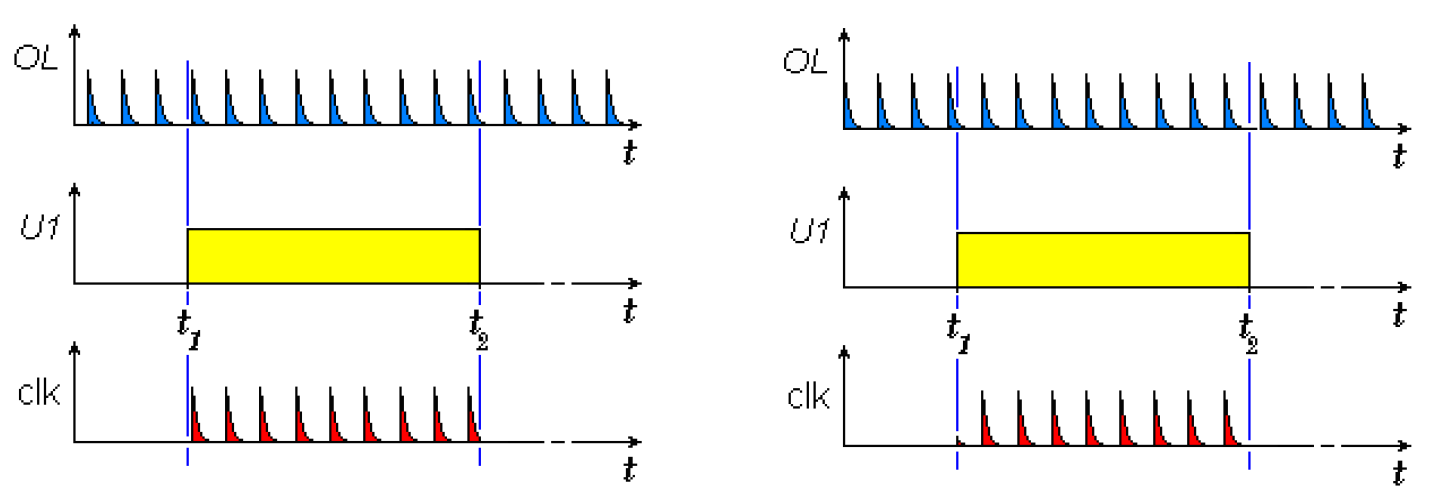
\includegraphics[scale = 0.4]{incertezza da mancanza di sincronismo casi.PNG}
\end{figure}

Nel caso a sinistra viene contato N = 9, invece nel caso a destra N = 8. \newline 

Come nei casi precedenti, $t_2 - t_1$ hanno la stessa durata nell'U1 ($t_2 - t_1$ può essere chiamato anche periodo di finestra) 
ma sono posizionati in modo diverso rispetto ai segnali di OL, 
quindi si crea incertezza in mancanza di sincronismo. \newline

Di seguito, tutti i quattro casi possibili riguardo al sincronismo: 

\begin{figure}[h]
    \centering
    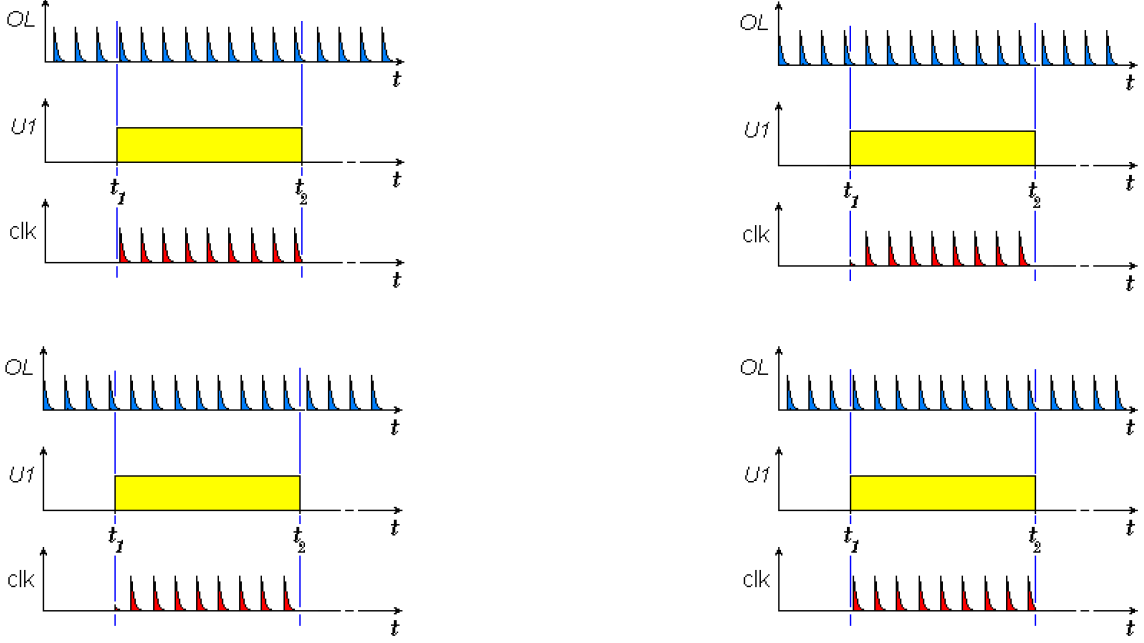
\includegraphics[scale = 0.5]{Casi possibili in mancanza di sincronismo tra U1 e OL.PNG}
\end{figure}

Analizzando tutti e quattro i casi di esempio, notiamo che l'incertezza di N in: 

{
    \Large 
    \begin{equation}
        t_2 - t_1 = N \tau
    \end{equation}
} 

è di: 

{
    \Large 
    \begin{equation}
        \Delta N = \pm 1
    \end{equation}
} 

e questo per definizione perchè, essendo N un numero razionale, non si può misurare $t_2 - t_1$ sotto il tempo $\tau$. \newline 

\newpage 

\subsection{Incertezza complessiva}
\footnote{Slide della prof | SDME 4 Strumenti numerici indicatori - parte I | pag 16 - 17 \\  
Appunti | 2025-04-11 | pag 12 - 14 | 2025-04-15 | pag 2 - 3}

Per concludere, l'incertezza di: 

{
    \Large 
    \begin{equation}
        t_2 - t_1 = N \tau
    \end{equation}
} 

è: 

{
    \Large 
    \begin{equation}
        \frac{\Delta (t_2 - t_1)}{t_2 - t_1}
        = 
        \frac{\Delta \tau}{\tau} 
        + 
        \frac{\Delta N}{N}
    \end{equation}
}

dove $\frac{\Delta \tau}{\tau} $ dipende dalla bontà dell'oscillatore locale, 
che se l'oscillatore fa il suo dovere (cit. Francescangeli): 

{
    \Large 
    \begin{equation}
        \frac{\Delta \tau}{\tau} = 0
    \end{equation}
}

Sapendo che: 

{
    \Large 
    \begin{equation}
        \Delta N = \pm 1
    \end{equation}
}

e riscrivendo la seguente equazione come: 

{
    \Large 
    \begin{equation}
        \begin{split}
        t_2 - t_1 &= N \tau 
        \\
        &\updownarrow
        \\ 
        N &= \frac{t_2 - t_1}{\tau} 
        \end{split}
    \end{equation}
} 

allora $\frac{\Delta N}{N}$ vale: 

{
    \Large
    \begin{equation}
        \begin{split}
            \frac{\Delta N}{N} 
            &=
            \frac{\pm 1}{N}
            \\
            &= 
            \frac{\pm \tau}{(t_2 - t_1)}
        \end{split}
    \end{equation}
}

Quindi l'incertezza di N dipende dal rapporto tra il periodo del campione dell'OL 
e la durata dell'intervallo da misurare. \newline 

Miglioriamo la misura se: 

{
    \Large 
    \begin{equation}
        t_2 - t_1 > \tau
    \end{equation}
}

o, in altri termini, ci serve sia un oscillatore locale che misura tempi molto brevi 
e anche un registro molto elevato. \newline 

\newpage 

\section{Grande capacità contatore e display}
\footnote{Slide della prof | SDME 4 Strumenti numerici indicatori - parte I | pag 18 \\  
Appunti | 2025-04-15 | pag 3}

Un altro vantaggio degli strumenti numerici digitali, cioè quelli che si usano spesso oggigiorno, è 
quello di avere un grosso display e un contatore molto elevato: 

\begin{figure}[h]
    \centering
    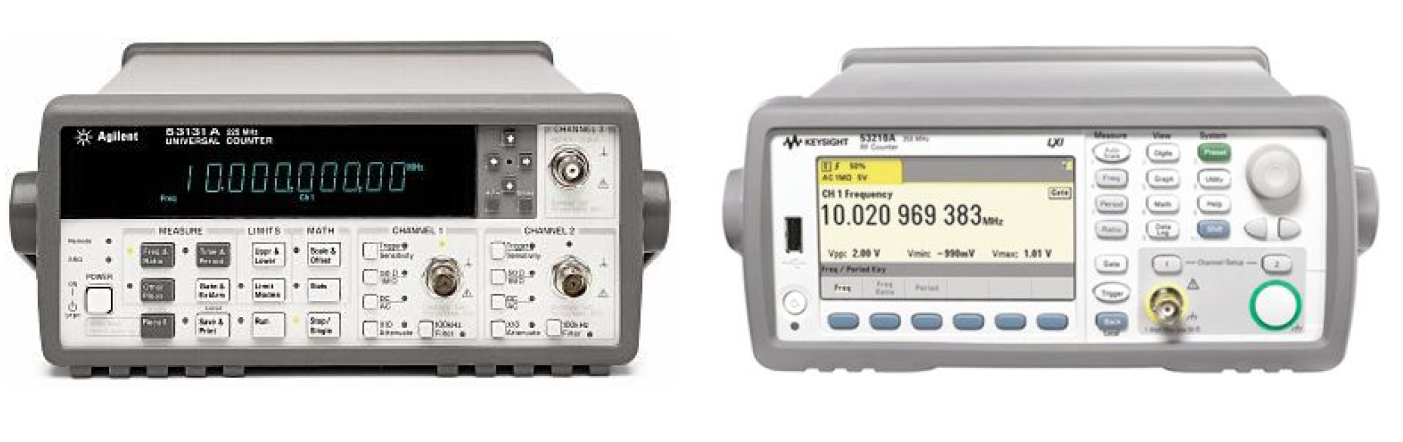
\includegraphics[scale = 0.4]{Strumenti moderni.PNG}
\end{figure}

I contatori di strumenti di misura da banco arrivano a 30 bit, cioè 1 miliardo di valori. \newline 

\newpage 

\section{Segnali analogici e circuito di trigger}
\footnote{Slide della prof | SDME 4 Strumenti numerici indicatori - parte I | pag 19 \\  
Appunti | 2025-04-15 | pag 3 }

Per i segnali analogici, si può modificare l'architettura del circuito dell'intervallometro numerico che funziona solo con segnali digitali: 

\begin{figure}[h]
    \centering
    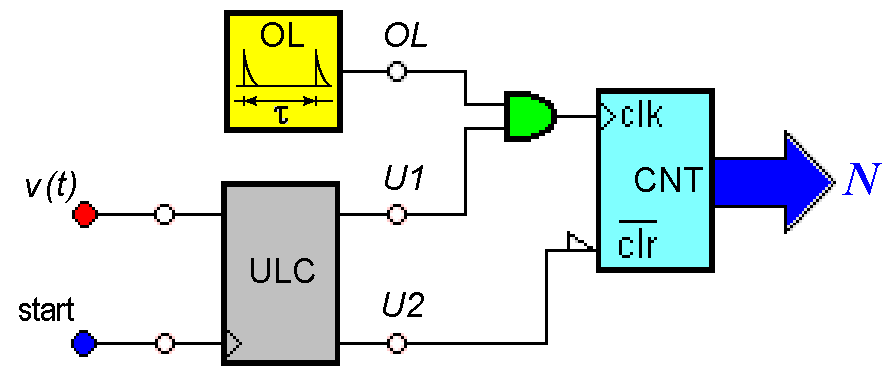
\includegraphics[scale = 0.4]{OL GATE CNT.png}
\end{figure} 

per adattarlo a segnali analogici. \newline 

Per fare ciò, si aggiunge un circuito di trigger al pin di v(t):

\begin{figure}[h]
    \centering
    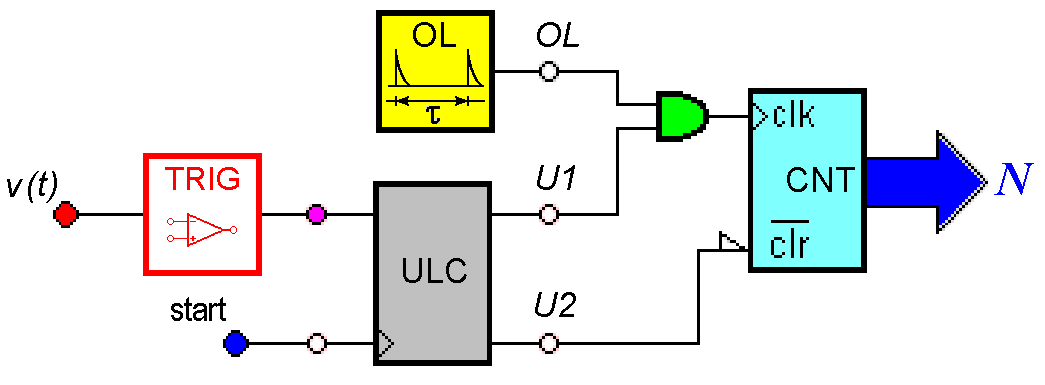
\includegraphics[scale = 0.8]{seganli analogici e circuito di trigger.png}
\end{figure} 

Il circuito di trigger (quello in rosso nella figura) può essere chiamato anche blocco di condizionamento del segnale 
perchè il segnale analogico v(t) a sinistra (quindi in ingresso) del Trigger deve rispecchiare certi parametri in modo che 
il circuito dell'intervallometro numerico (cioè dal pin rosa in poi in figura) possa iniziare la misura. \newline 

\newpage 

\subsection{Funzionamento del trigger}
\footnote{Slide della prof | SDME 4 Strumenti numerici indicatori - parte I | pag 20 \\  
Appunti | 2025-04-15 | pag 4}

Per la spiegazione del funzionamento del trigger, consideriamo un caso ideale. \newline 

Consideriamo il seguente circuito e la visualizzazione delle tensioni nei vari pin del circuito: 

\begin{figure}[h]
    \centering
    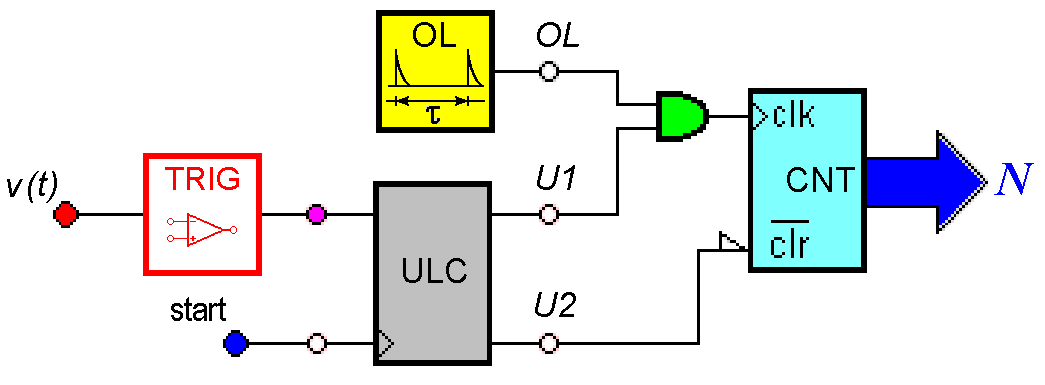
\includegraphics[scale = 0.6]{seganli analogici e circuito di trigger.png}
    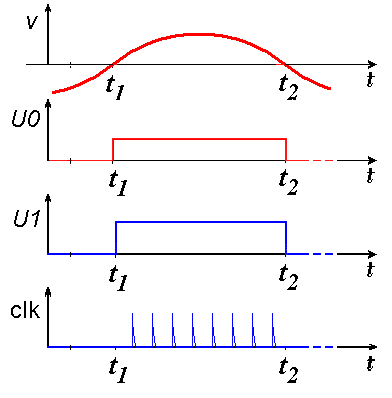
\includegraphics[scale = 1]{tensioni nei pin con intervallometro con circuito di trigger.png}
\end{figure} 

Per U0 si intende il pin di uscita dal trigger, quello rosa in figura. \newline 

Il trigger dell'intervallometro porta la sua uscita allo stato vero quando nel segnale v(t) si verifica una certa condizione. \newline 

Poi, l'uscita del trigger ritorna falsa, quando si verifica un'altra condizione. \newline 

Entrambe le condizioni sono selezionabili dall'operatore. \newline 

\newpage 

\subsection{Regolazione del trigger}
\footnote{Slide della prof | SDME 4 Strumenti numerici indicatori - parte I | pag 21 - 22 \\  
Appunti | 2025-04-15 | pag 4 - 5}

Il trigger dell'intervallometro porta la sua uscita allo stato vero quando nel segnale v(t) si verifica una certa condizione. \newline 

Negli strumenti digitali moderni si possono scegliere diverse caratteristiche che il segnale analogico deve avere per attivare il circuito di trigger 
(ricordando il seminario svolto in classe dallo Rohde \& Schwarz sugli oscilloscopi odierni). \newline 

Qui si riportano le caratteristiche dei segnali fondamentali per attivare il circuito di trigger, che sono: 

\begin{itemize}
    \item level, cioè il livello minimo che deve avere il segnale analogico
    \item slope, cioè la pendenza minima che deve avere il segnale analogico
\end{itemize}

Il level e lo slope possono essere configurati in modo che le impostazioni siano di fine o di inizio, dipende tutto dallo strumento. \newline 

Dato per esempio questo multimetro con due ingressi: 

\begin{figure}[h]
    \centering
    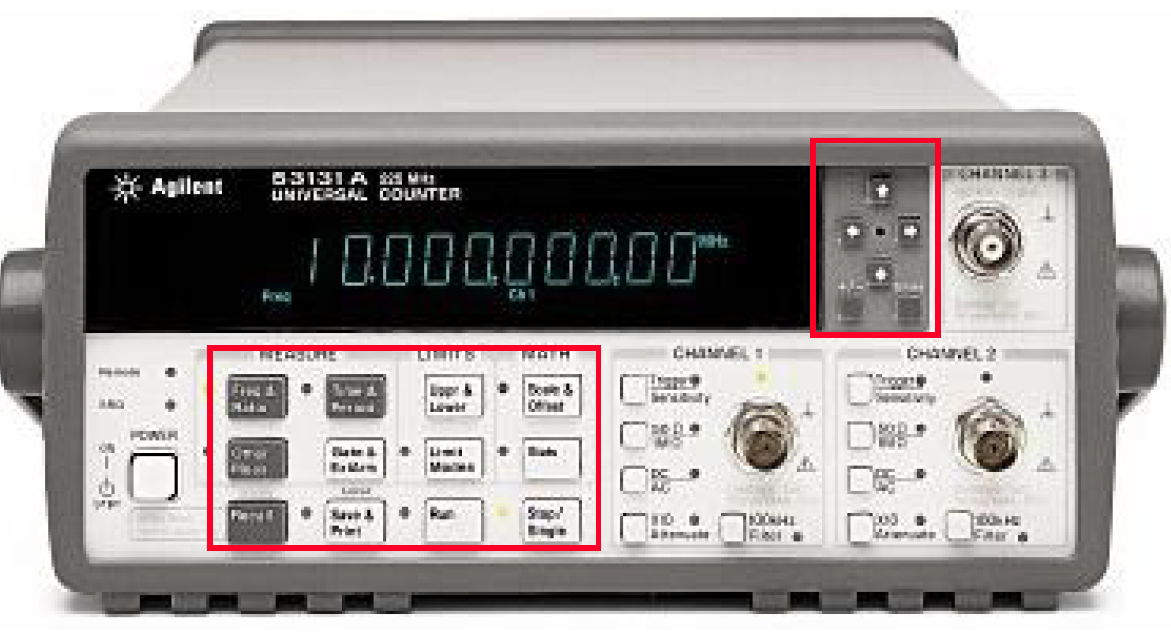
\includegraphics[scale = 0.6]{Level e slope in un multimetro da banco 1.PNG}
\end{figure} 

si può selezionare il level e slope differenti per i rispettivi ingressi. \newline 

In strumenti un po' più datati, si potevano cambiare questi parametri con delle manopole analogiche: 

\begin{figure}[h]
    \centering
    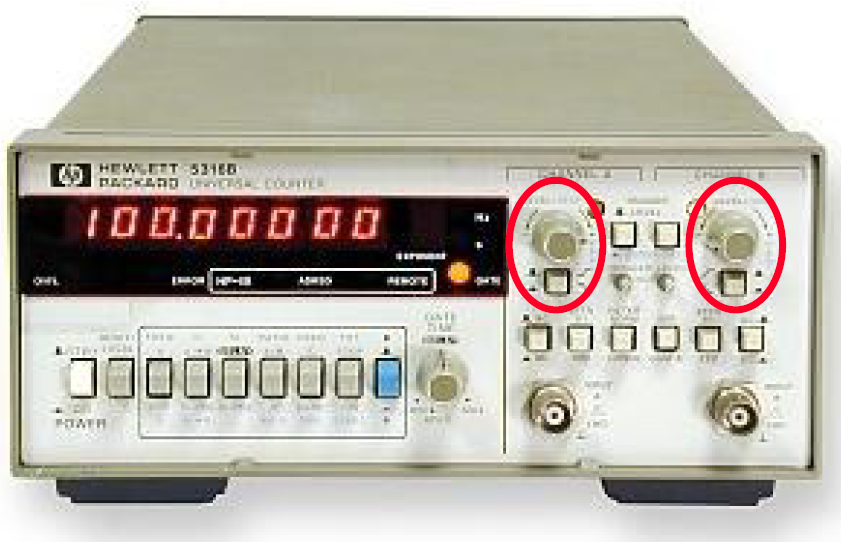
\includegraphics[scale = 0.6]{Level e slope in un multimetro da banco 2.PNG}
\end{figure} 

\newpage 

\section{Periodometro numerico: schema di principio}
\footnote{Slide della prof | SDME 4 Strumenti numerici indicatori - parte I | pag 23 \\  
Appunti | 2025-04-15 | pag 5}

Possiamo considerare questo circuito: 

\begin{figure}[h]
    \centering
    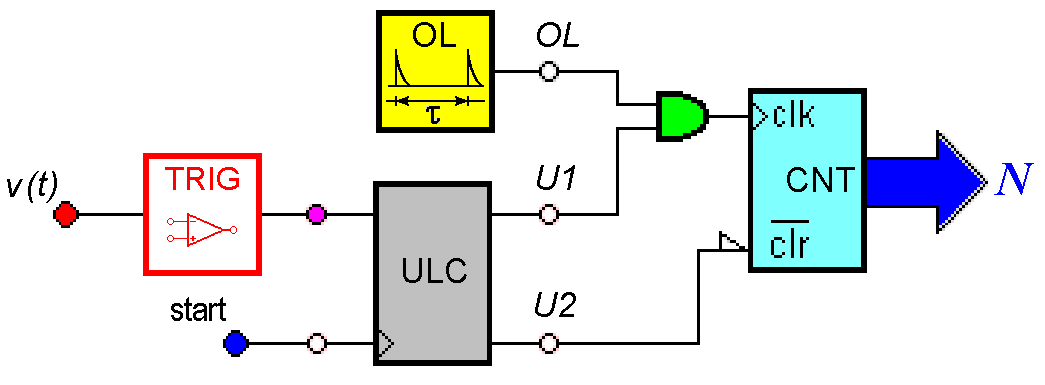
\includegraphics[scale = 0.6]{seganli analogici e circuito di trigger.png}
\end{figure} 

cioè un intervallometro con un circuito di trigger, se il trigger opera come un blocco di divisore di frequenza, 
cioè ciclicamente rende la sua uscita vera quando v(t) assume un certo stato e la riporta falsa quando v(t) torna ad assumere lo stesso stato. \newline 

\newpage 

\subsection{Periodometro - Trigger F/2}
\footnote{Slide della prof | SDME 4 Strumenti numerici indicatori - parte I | pag 24 \\  
Appunti | 2025-04-15 | pag 5 - 6}

Per fare ciò che è richiesto, cioè che il trigger ciclicamente rende la sua uscita vera quando v(t) assume un certo stato e la riporta falsa quando v(t) torna ad assumere lo stesso stato, 
ci è molto utile il flip-flop D. \newline 

Dalla tabella di verità del flip-flop D: 

\begin{figure}[h]
    \centering
    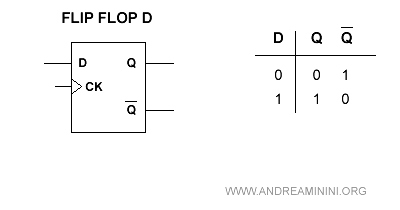
\includegraphics[scale = 0.8]{flip-flop-d-tavola-di-verita.jpg}
\end{figure} 

possiamo visualizzare la componentistica del circuito di trigger e l'andamento nei pin nel tempo: 

\begin{figure}[h]
    \centering
    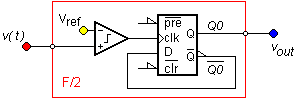
\includegraphics[scale = 2]{Periodometro esploso.png}
    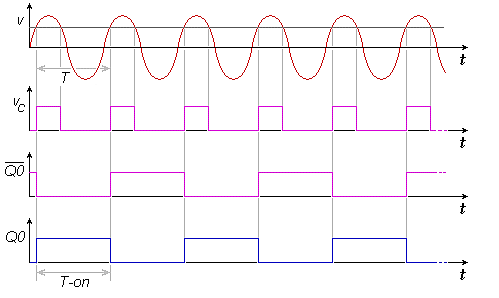
\includegraphics[scale = 1.5]{Andamento dei pin nel periodometro.png}
\end{figure}

Consideriamo il segnale di ingresso v(t) perfettamente sinusoidale e periodico. \newline 

Nella figura, $V_c$ è l'andamento del segnale del pin di clock clk nel flip-flop, 
e v corrisponde all'andamento del segnale analogico sinusoidale v(t). \newline 

L'obbiettivo del periodometro è quello di misurare T, il famoso $t_2 - t_1$, cioè il tempo di periodo della sinusoide. \newline 

Come si può osservare dal circuito, il comparatore è collegato al clock, 
quindi quando il segnale v(t) diventa maggiore della soglia $v_{ref}$, clk diventa alto, 
quando v(t) si abbassa di $v_{ref}$, $v_c$ diventa basso. \newline 

Il periodo in cui $v_c$ rimane alto è proprio T/2. \newline 

Essendo un flip-flop D, Q0 rimane alto finché non riceve un altro impulso alto da clk, quindi dal comparatore. \newline 

Q0 rimane alto per un periodo T-on. \newline 

Rispetto all'intervallometro numerico, non è l'oscillatore locale che aumenta il contatore, 
bensì il segnale analogico v(t). \newline 

\newpage 

\subsection{Periodometro: principio della misurazione}
\footnote{Slide della prof | SDME 4 Strumenti numerici indicatori - parte I | pag 25 \\  
Appunti | 2025-04-15 | pag 6}

Partendo dal segnale di cui si vuole misurare il periodo, 
si costruisce un segnale di servizio che ha la caratteristica di presentare un 
$T_{on}$ pari al periodo incognito: 

\begin{figure}[h]
    \centering
    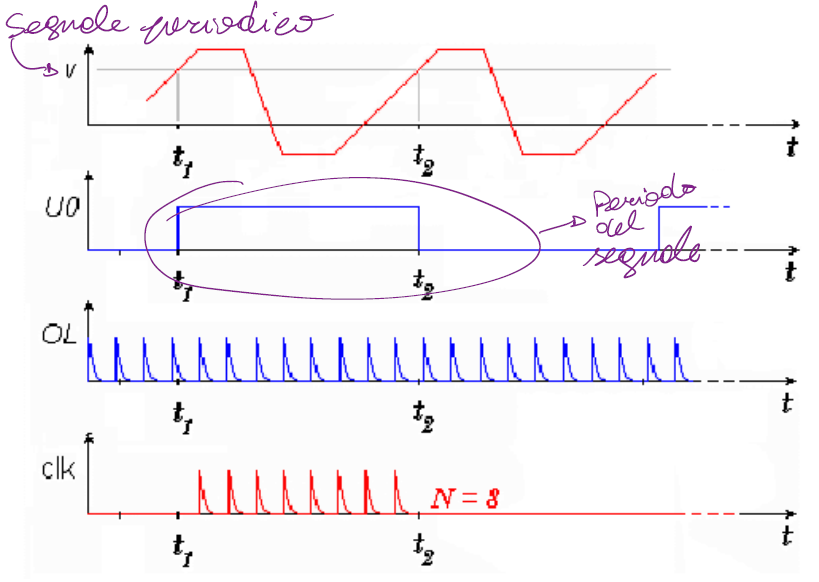
\includegraphics[scale = 1]{Periodo di un segnale in un periodometro.PNG}
\end{figure}

A questo punto basta misurare la durata dell'intervallo corrispondente al $T_{on}$ mediante 
le procedure già discusse per l'intervallometro. \newline 

\newpage 

\section{Periodometro}
\footnote{Slide della prof | SDME 4 Strumenti numerici indicatori - parte I | pag 26 \\  
Appunti | 2025-04-15 | pag 6}

Il principio di funzionamento del periodometro e dell'intervallometro è lo stesso, 
ma si misurano due cose diverse: 

\begin{itemize}
    \item nel periodometro si vuole misurare l'intervallo T del segnale 
    \item nell'intervallometro si vuole misurare un segnale alto-basso generico
\end{itemize}

Quindi, dato lo schema del periodometro e degli andamenti dei segnali, si può spiegare il principio di funzionamento del periodometro: 

\begin{figure}[h]
    \centering
    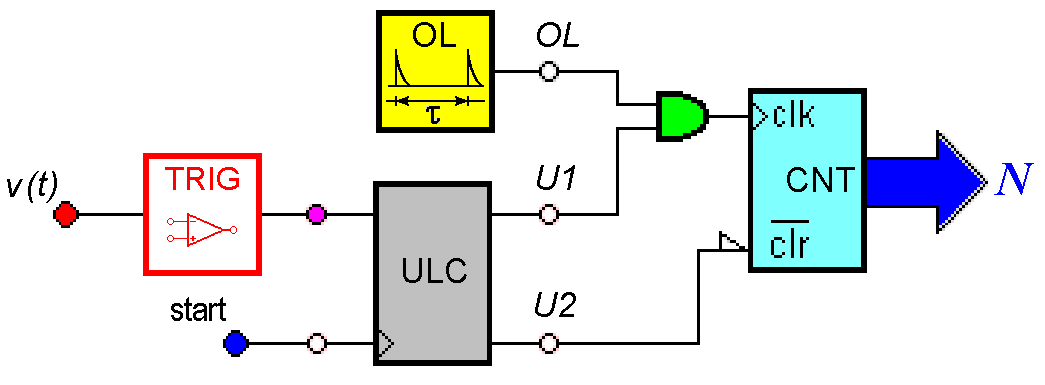
\includegraphics[scale = 0.5]{seganli analogici e circuito di trigger.png}
    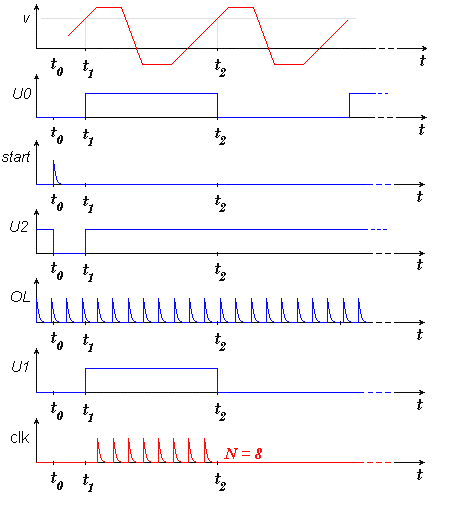
\includegraphics[scale = 1]{tensioni in un periodometro.png}
\end{figure}

Quindi stesse considerazioni dell'intervallometro. \newline 

T, cioè periodo del segnale v(t), si misura come: 

{
    \Large 
    \begin{equation}
        T = N \tau
    \end{equation}
}

e l'incertezza di T è: 

{
    \Large 
    \begin{equation}
        \frac{\Delta T}{T} 
        = 
        \frac{\Delta \tau}{\tau}
        +
        \frac{\Delta N}{N}
    \end{equation}
}

\newpage 

\subsection{Incertezza complessiva}
\footnote{Slide della prof | SDME 4 Strumenti numerici indicatori - parte I | pag 27}

La seguente espressione possiamo scriverla anche come: 

{
    \Large 
    \begin{equation}
        \begin{split}
            T &= N \tau
            \\ 
            &\updownarrow
            \\
            N &= \frac{T}{\tau}
        \end{split}
    \end{equation}
}

e sapendo che, dalle considerazione svolte sull'intervallometro: 

{
    \Large 
    \begin{equation}
        \Delta N = \pm 1
    \end{equation}
}

allora possiamo esprimere $\frac{\Delta N}{N}$ come:

{
    \Large 
    \begin{equation}
        \begin{split}
            \frac{\Delta N}{N}
            &= 
            \pm
            \frac{1}{N}
            \\ 
            &= 
            \pm 
            \frac{\tau}{N}
        \end{split}
    \end{equation}
}

$\frac{\Delta \tau}{\tau}$ dipende dalla qualità del campione di tempo utilizzato, cioè dall'oscillatore locale, 
invece $\frac{\Delta N}{N}$ dipende dal rapporto fra il campione del tempo ed il periodo del segnale sotto misurazione. \newline 

\newpage

\subsection{Periodometro: incertezza da disturbi su $v_x$ - jitter}
\footnote{Slide della prof | SDME 4 Strumenti numerici indicatori - parte I | pag 28 - 29 \\  
Appunti | 2025-04-15 | pag 7 - 9 | 2025-06-23 Ricevimento | pag 1, 4}

Come studiato nel corso di Segnali determinati e Aleatori, il rumore è indipendente rispetto al segnale che vogliamo misurare. \newline 

Il rumore è diverso istante per istante. \newline 

Per jitter si intende un rumore che si sovrappone al segnale utile e che si trova nell'intorno del segnale. \newline 

Considerano un segnale utile privo di rumore: 


\begin{figure}[h]
    \centering
    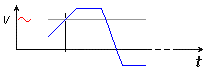
\includegraphics[scale = 3]{Segnale utile.png}
\end{figure}

si può sommare un rumore: 

\begin{figure}[h]
    \centering
    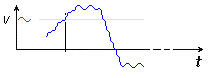
\includegraphics[scale = 3]{segnale utile con rumore.png}
\end{figure}

Da un segnale senza rumore in cui ogni tempo t è definibile un suo punto ben noto, 
il rumore modifica il comportamente del segnale privo di rumore. \newline 

Visto che il livello di trigger è costante, il segnale sovrapposto al rumore potrebbe eccitare il trigger più di una volta. \newline 

Allora si sceglie di impostare il trigger non su un tempo t definito, bensì su un intervallo $\hat{t}$. \newline 

Quindi quanto vale il segnale al tempo $\hat{t}$  ? 

\begin{figure}[h]
    \centering
    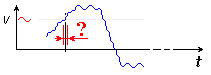
\includegraphics[scale = 3]{segnale utile con rumore al tempo t.png}
\end{figure}

Se si considera v(t) il segnale senza rumore, l($\hat{t}$) il livello impostato nel trigger, 
e n($\hat{t}$) il segnale di rumore all'istante $\hat{t}$, allora si può recuperare v(t) con: 

\begin{figure}[h]
    \centering
    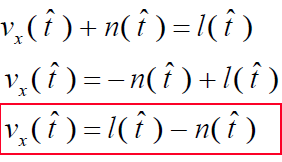
\includegraphics[scale = 1]{Passaggi algebrici per recuperare il segnle v_x.PNG}
\end{figure}

\newpage 

\begin{tcolorbox}
    Sembrano semplici passaggi algebrici banali, ma non sono così scontati. \newline 
    Sono valide queste relazioni se il rumore è solo additivo.  
\end{tcolorbox}

Dato l'andamento del segnale $v_x (t)$ è possibile scegliere un intervallo dei tempi $\Delta t$ in cui si linearizzarà il segnale $v_x (t)$: 

\begin{figure}[h]
    \centering
    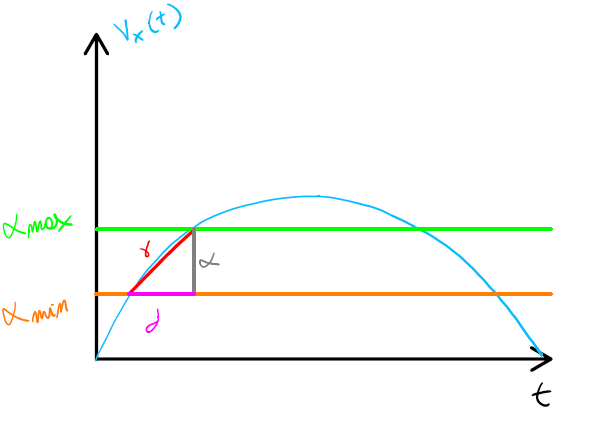
\includegraphics[scale = 1]{Andamento di un segnale senza rumore.PNG}
\end{figure}

Così facendo, si costruirà un triangolo rettangolo composto da: 

\begin{itemize}
    \item cateto $\alpha$ 
    \item cateto $\Delta t$
    \item ipotenusa, che collega i punti $\alpha_{max}$ e $\alpha_{min}$
\end{itemize}

ma non sappiamo a priori il valore che ha l'ipotenusa. \newline 

Dalla trigonometria, possiamo scrivere: 

{
    \Large
    \begin{equation}
        \begin{cases}
        \Delta_t = \text{ ipotenusa } \cdot \cos \alpha
        \\ 
        \alpha = \text{ ipotenusa } \cdot \sin \alpha     
        \end{cases}
    \end{equation}
}


allora possiamo esprimere la seguente equazione: 

{
    \Large 
    \begin{equation}
        \begin{split}
            \frac{\Delta_t}{\alpha}
            &= 
            \frac{\text{ ipotenusa } \cdot \cos \alpha}{\text{ ipotenusa } \cdot \sin \alpha  } 
            \\
            &=
            \frac{\cos \alpha}{\sin \alpha}
            \\
            &= 
            \tan(\alpha)
            \\
            &=
            \text{ SR}
        \end{split}
    \end{equation}
}

dove SR indica la pendenza dell'ipotenusa. \newline 

Per recuperare il segnale v(t), è meglio porsi nel punto massimo in cui si ha una pendenza maggiore del segnale. \newline 

SR prende il nome di pendenza o slew rate e si misura in $[\frac{V}{s}]$. \newline 

\newpage 
